\documentclass{report}
\usepackage[utf8]{inputenc}
\usepackage[portuguese]{babel}
\usepackage{graphicx}


\title{PL - Processamento de Linguagens\\Report 2007: vamos escrever relatórios}
\author{a61030 - Diogo Alves\\a61075 - Ricardo Branco\\a61084 - Helder Gonçalves}
\date{2 de Junho de 2013}


\begin{document}

\maketitle

\tableofcontents

\chapter{Resumo}

Neste trabalho temos como objetivo criar um analisador léxico e um sintático, que "processa"/analisa o texto, apanhando as palavras reservadas, e de seguida verifica se a estrutura do relatório está bem construida. Enquando analisa o texto vai guardando-o em estruturas de dados, e em listas ligadas para separar o código html do código latex, convertendo e criando por fim ficheiros HTML e/ou LaTeX com o nosso relatório convertido para cada uma das linguagens. 


\chapter{Introdução}

Para o segundo Trabalho Prático da Unidade Curricular de Processamento de Linguagens, a nossa escolha foi o enunciado 3 que tem como titulo: "Report 2007: vamos escrever relatórios".
Neste projeto, pretende-se que seja criado um compilador capaz de "converter" uma relatório escrito numa linguagem criada por nós, e já usada no trabalho prático 1 para a linguagem HTML ou/e LaTeX.  
Portanto, neste documento irão estar presentes as nossas decisões, a estruturação do projecto, bem como as explicações e funcionamento do mesmo.



\chapter{Sintaxe da Nossa Linguagem}

Nós, como referido anteriormente, estamos a "continuar" o trabalho realizado no Trabalho Prático 1 (TP1) e por isso a sintaxe da linguagem manteve-se a do trabalho anterior, que é a seguinte:

\begin{figure}[h]
\centering
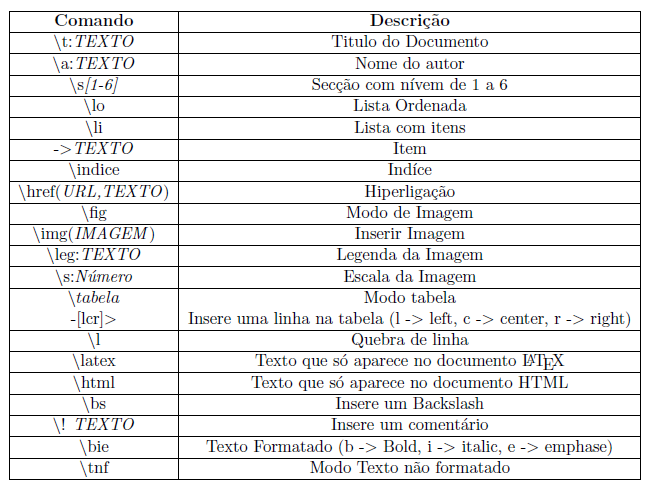
\includegraphics[scale=0.7]{sintaxe.PNG}
\caption{Sintaxe da Linguagem}
\label{Linguagem}
\end{figure}


\chapter{Estruturação do Trabalho}

Este trabalho consiste em dois analisadores, um lexico, feito em flex que irá "apanhar" as palavras reservadas na nossa linguaguem e passar a informação do que reconheceu para o analisador sintático, feito em yacc, que irá verificar se a gramática obtida do documento que está a ser analisado está correta.
Depois disto, e no yacc, gravamos os dados em estruturas de dados. Por fim, vamos buscar os dados a essas estruturas e criamos um ficheiro HTML e/ou LaTeX com a nossa linguagem convertida para essas linguagens.

Fazendo um esquema ficaria assim:

\begin{figure}[h]
\centering
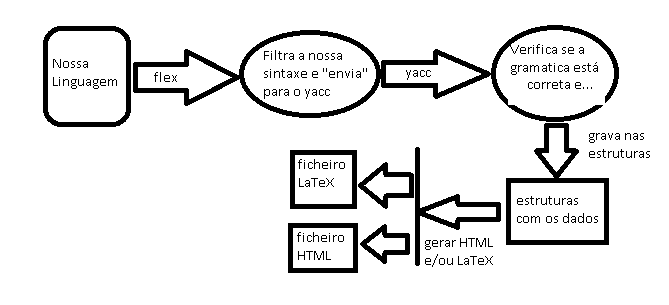
\includegraphics[scale=0.6]{esq.png}
\caption{Esquema da estrutura}
\label{Estrutura}
\end{figure}



\chapter{Conclusão}

Este trabalho prático permitiu-nos consolidar os conhecimentos obtidos nas aulas uma vez que precisamos de tudo o que temos vindo a dar, a forma como estruturar o compilador, como funcionava a gramática disponibilizada pelo docente, o que era suposto os analisadores lexico e semantico fazerem, como funcionavam e interagiam, e nesse aspeto as aulas ajudaram bastante pois tudo foi explicado lá.
O nível de dificuldade neste trabalho foi um pouco maior que no primeiro, o que era de esperar, e foi facilitado pelo facto de termos já grande parte da gramática, apenas tendo de fazer algumas alterações e acrescentar algumas derivações para ser compativel com o nosso primeiro trabalho.
O facto de escolher-mos este enunciado também facilitou, porque no primeiro trabalho já tinhamos definido a sintaxe da nossa linguagem e então apenas tivemos de alterar um pouco o flex e não pensar em toda a sintaxe/gramática novamente, já tinhamos usado estruturas de dados no primeiro trabalho e foi só altera-las minimamente e aplica-las neste trabalho, o que nos poupou bastante tempo e trabalho.
A nossa satisfação perante o que foi produzido neste trabalho é positiva, uma vez que ficamos a perceber melhor a estruturação do compilador dividindo o analisador em analisador lexico e sintatico, colocando depois um programa em C a fazer a gestão dos dados e escrever nos ficheiros HTML e LaTeX nas respetivas linguagens. 




\end{document}
